\chapter{模形式与自守表示}\label{L6}
\lecturedate{2020/03/04}
\sourcepage{43}
回忆，我们希望按照如下过程建立对应：
\begin{figure}[H]\centering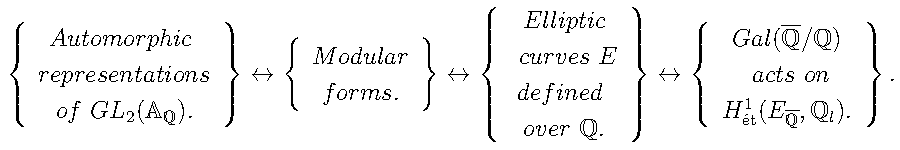
\includegraphics[width=0.7257\paperwidth]{images/L6-p043-correspondence.pdf}\end{figure}
因此，现在该讨论模形式了。取$G=\GL_2$。
\section{模形式}\label{L6S1}\idx{模形式}
模形式\znote{模形式可以理解为「$\mathcal H$ 上变换规律由权 $k$ 决定的全纯函数」。权 $k$ 的几何含义是：$f(z)(\mathrm dz)^{k/2}$ 在 $\Gamma$-作用下不变，因此模形式是模曲线上的截面；等价地，$k$ 对应 $\SO_2(\R)$ 的一个特征。按 nLab 的说法，模形式常被称为「经典自守形式」，第 2 节将把它对应到 $\mathcal A_0(G)$ 中的向量。[来源：nLab "modular form"，\url{https://ncatlab.org/nlab/show/modular+form}（Last revised 2025-03-13；2026-11-14 访问）。]}是定义在上半平面$\mathcal H:=\{z\in\C\mid\Impart z>0\}$上的全纯函数。另一方面，$G(\R)^+=\{g\in G(\R)\mid\det g>0\}$通过如下方式作用于$\mathcal H$：
\[g=\begin{pmatrix}a&b\\c&d\end{pmatrix}\in G(\R)^+,\qquad g(z):=\frac{az+b}{cz+d}.\]
容易验证，$g_2(g_1(z))=(g_2g_1)(z)$，且\[\Impart(g(z))=\frac{\det g}{|cz+d|^2}\Impart z.\]于是，由$g\mapsto g(i)$得到同构\[\SL_2(\R)/\SO_2(\R)\xrightarrow{\sim}\mathcal H.\]因此，$\mathcal H$上的函数$f$可转化为$\SL_2(\R)$上的函数$F$，定义为$F(g)=f(g(i))$。
\sourcepage{44}
函数$F$还在右$\SO_2(\R)$作用下不变。

不过，正如\eref{引理}{L4S2O2}所示，我们要描述的是$\GL_2(\R)^+$上左$\Gamma$-不变的函数，其中$\Gamma$为某个同余子群\znote{同余子群指 $\SL_2(\Z)$ 中由「模 $n$ 同余条件」切出的子群；等价地，它是某个投影 $\SL_2(\Z)\to\SL_2(\Z/n\Z)$ 之下子群的原像。主同余子群 $\Gamma(n)$ 正是这个投影的核；另有两个常用特例：$\Gamma_0(N)$ 要求下三角元 $\equiv0\pmod N$，$\Gamma_1(N)$ 还要求对角元 $\equiv1$。它们都有限指数，因此 $\Gamma\backslash\mathcal H$ 是复曲线。[来源：nLab "congruence subgroup"，\url{https://ncatlab.org/nlab/show/congruence+subgroup}（Last revised 2026-05-25；2026-11-14 访问）。]}。它形如$\Gamma=G(\Q)\cap(G(\R)^+U)$，其中$U\subseteq G(\A^f)$为满足$\det U=\widehat{\Z}^\times$的紧开子群。可假定$U\subseteq G(\widehat{\Z})$，此时$\Gamma\subseteq\SL_2(\Z)$。

下面取$\Gamma$为Hecke同余子群\znote{「Hecke 同余子群」得名于它对 Hecke 算子封闭：对每个 $n\geq1$，双陪集 $\Gamma_0(N)\begin{pmatrix}n&0\\0&1\end{pmatrix}\Gamma_0(N)$ 给出算子 $T_n$，它保持 $M_k(N)$ 并把 Fourier 系数重新组合；各个 $T_n$ 两两交换，其公共本征函数就是 Hecke 本征形式。本讲只用到 $T_p$ 给出的局部因子，第 8 讲将系统讨论 Hecke 代数。[来源：D. Bump, \textit{Automorphic Forms and Representations}, Cambridge Studies in Advanced Mathematics 55, Cambridge University Press, 2004（本讲参考文献）。]}。设$N$为正整数，
\begin{equation}\tag{1.1}\label{L6eq11}
\Gamma_0(N)=\left\{\begin{pmatrix}a&b\\c&d\end{pmatrix}\in\SL_2(\Z)\ \middle|\ c\equiv0\pmod N\right\}.
\end{equation}
$\Gamma$是与下列紧开子群$U^\Gamma$相对应的同余子群：
\begin{equation}\tag{1.2}\label{L6eq12}
U^\Gamma=U^N=\prod_p\left\{\begin{pmatrix}a&b\\c&d\end{pmatrix}\in\GL_2(\Z_p)\ \middle|\ \ord_p(c)\geq\ord_p(N)\right\}.
\end{equation}
注意，$\mathbb P^1(\Q)\cong G(\Q)/B(\Q)$，其中$B(\Q)$是$G(\Q)$中上三角矩阵组成的Borel子群。
% [Tutor Note: 原书 p44 把 $B(\Q)$ 说成 $G(\R)$ 中上三角矩阵组成的子群，译文按 $B(\Q)\subseteq G(\Q)$ 处理。]
同构由
\[\GL_2(\Q)\ni\begin{pmatrix}a&b\\c&d\end{pmatrix}\longmapsto[a:c]\]
诱导。$\Gamma$的一个\textbf{尖点}是$\mathbb P^1(\Q)$中的一个$\Gamma$-轨道。若$N=1$，则$\Gamma=\SL_2(\Z)$，只有一个尖点$\infty$。一般地，尖点个数为$|\Gamma\backslash\SL_2(\Q)/B_{\SL_2}(\Q)|$，这是有限的；添加这些尖点便可将$\Gamma\backslash\mathcal H$紧化：
\[\overline{\Gamma\backslash\mathcal H}=\Gamma\backslash(\mathcal H\cup\Q\cup\{\infty\}).\]
\idx{尖点}
\originalnumber{1}
\begin{definition}{全纯模形式}\label{L6S1O1}
$\Gamma$的一个\textbf{全纯模形式}是$\mathcal H$上的全纯函数$f$，满足以下两个性质：
\begin{itemize}
\item （自守性）对任意$\gamma=\begin{pmatrix}a&b\\c&d\end{pmatrix}\in\Gamma$，有$f(\gamma(z))=(cz+d)^k f(z)$，其中$k$为正整数，称为$f$的\textbf{权}；
\sourcepage{45}
\item （全纯性）$f$在$\Gamma$的每个尖点处都全纯。
\end{itemize}
当$\Gamma=\Gamma_0(N)$时，$N$称为$f$的\textbf{级}。若$f$还在每个尖点处为零，就称它为\textbf{尖点形式}，或称$f$具有尖点性。
\end{definition}
\idx{权（模形式）}\idx{级（模形式）}\idx{尖点形式}
\originalnumber{2}
\begin{note}[L6S1O2]
\begin{enumerate}
\item 若$k$为奇数，则$f$必为零，因为$\begin{pmatrix}-1&0\\0&-1\end{pmatrix}\in\Gamma$。
\item 因$t=\begin{pmatrix}1&1\\0&1\end{pmatrix}\in\Gamma$，有$f(z+1)=f(z)$。因此$f$实际上可看成带状区域$\{x+iy\mid-1/2\leq x\leq1/2,\ y>0\}$上的函数。
\item 作变量代换$z\mapsto q=e^{2\pi iz}$，得到$f$在$q=0$附近的Laurent展开\znote{$q=e^{2\pi iz}$ 是尖点 $i\infty$ 处的局部坐标：它把上半平面映到去心圆盘，$z\to i\infty$ 对应 $q\to0$，而带形区域 $\{0<\Re z<1\}$ 映到 $0<|q|<1$。所谓「$f$ 在尖点全纯」，就是它的 Laurent 展开没有负幂项。于是模形式等价于一列满足自守关系的系数 $a_n$，Hecke 本征值与 $L$ 函数这些算术信息全部装在这一列系数里。[来源：nLab "modular form"，\url{https://ncatlab.org/nlab/show/modular+form}（Last revised 2025-03-13；2026-11-14 访问）。]}
\[f(z)=f(q)=\sum_n a_nq^n.\]
由于$f$在$i\infty$处全纯，$f(q)$在$q=0$处全纯，故上式中$n<0$时$a_n=0$。于是$f$有Fourier级数展开
\[f(z)=f(q)=\sum_{n\geq0}a_n(f)q^n.\]
数列$\{a_n(f)\}$称为$f$在尖点$\infty$处的Fourier系数。
\item $f$为尖点形式，当且仅当它在每个尖点处的Fourier展开都满足$a_0(f)=0$。注意，每个尖点都可以通过$\SL_2(\Z)$的某个元素移到$\infty$。
\end{enumerate}
\end{note}
对$f\in M_k(\Gamma)$，若存在$n$和$C$，使当$y\to\infty$且$x$有界时，有$|f(x+iy)|\leq Cy^n$，就说$f$在尖点$i\infty$处\textbf{适度增长}。由Fourier展开，$f$在$i\infty$处适度增长，当且仅当它在$i\infty$处全纯。把其他尖点移到$\infty$，也可对它们定义同样的性质。
\sourcepage{46}
记$M_k(N)$为$\Gamma_0(N)$的所有全纯模形式组成的空间，$S_k(N)$为其中的尖点形式空间。这些复向量空间都是有限维的！此外，$\bigoplus_kM_k(N)$具有环结构，因为若$f_j\in M_{k_j}(N)$（$j=1,2$），则$f_1f_2\in M_{k_1+k_2}(N)$。
\needspace{4\baselineskip}\originalnumber{3}
\begin{example}\label{L6S1O3}\idx{Eisenstein级数}
对$k>1$，归一化Eisenstein级数\znote{Eisenstein 级数是「显式可算」的模形式：$G_4$ 与 $G_6$ 通过 $g_2=60G_4$、$g_3=140G_6$ 给出椭圆曲线的不变量，$\Delta=g_2^3-27g_3^2$ 与 $j=1728g_2^3/\Delta$ 由此把椭圆曲线的同构类读成模形式。第 7 讲会把这条线索变成「模形式 $\leftrightarrow$ 椭圆曲线」的对应；本节只需知道它是 $\Gamma_0(N)$ 上最具体的一类例子。[来源：nLab "Eisenstein series"，\url{https://ncatlab.org/nlab/show/Eisenstein+series}（Last revised 2014-03-26；2026-11-14 访问）。]}
\[E_{2k}(z)=\frac1{2\zeta(2k)}\sum_{\substack{(c,d)\in\Z^2\\(c,d)\ne(0,0)}}\frac1{(cz+d)^{2k}}\]
是$\SL_2(\Z)$的权$2k$模形式，其Fourier展开为
\[E_{2k}(z)=1-\frac{4k}{B_{2k}}\sum_{n=1}^{\infty}\sigma_{2k-1}(n)q^n.\]
这里$\zeta(s):=\sum_{n=1}^{\infty}n^{-s}$为Riemann的$\zeta$函数，$B_{2k}$为第$2k$个Bernoulli数，$\sigma_r(n):=\sum_{d\mid n}d^r$\znoteplain{判别这类公式对不对，最快的办法是代入最小的 $k$ 验算。$k=2$ 时 $B_4=-1/30$，$-4k/B_{2k}=8/(1/30)=240$，得 $E_4=1+240q+\cdots$；$k=3$ 时 $B_6=1/42$，$-4k/B_{2k}=-12/(1/42)=-504$，得 $E_6=1-504q+\cdots$。这两个展开必须与 $G_4=1+240q+\cdots$、$G_6=1-504q+\cdots$ 的系数一致。若误用第 $k$ 个 Bernoulli 数（$B_2=1/6$），$k=2$ 会算出 $48$，$q$ 展开随之出错——所以下标是 $B_{2k}$ 而非 $B_k$，符号也是负的。（上下文推断，无外部依据）}。
% [Tutor Note: 原书 p46 印作 $1+(-1)^k4k/B_k\cdot\sum\sigma_{2k-1}(n)q^n$ 并称「$B_k$ are the so-called nth Bernoulli number」；此处 Bernoulli 数下标应为 $2k$、符号应为负号，按标准写法 $1-4k/B_{2k}\sum\sigma_{2k-1}(n)q^n$ 处理（代入 $k=2,3$ 得 $E_4=1+240q+\dots$、$E_6=1-504q+\dots$ 可验证）。]
\end{example}
对偶数$k\geq4$，还满足$M_k(1)=\C E_k\oplus S_k(1)$。
\originalnumber{4}
\begin{example}\label{L6S1O4}\idx{Theta函数}
另一个重要例子是Theta函数。设$A$为$k$阶正定对称整数矩阵。假定$A$为偶矩阵，即对所有$x\in\Z^k$，$x^TAx$均为偶数，并且$\det A=1$。定义二次型$Q(x):=\tfrac12x^TAx$。级数
\[\theta_Q(z)=\sum_{x\in\Z^k}q^{Q(x)}=\sum_{n\geq0}a_n(Q)q^n,\]
其中$q=e^{2\pi iz}$，$a_n(Q)=|\{x\in\Z^k\mid Q(x)=n\}|$，是权$k/2$、级$1$的模形式。
\end{example}
\begin{exercise*}\label{L6S1EX}
证明：若$f\in M_k(n)$，则对任意满足$n\mid N$的$N$，都有$f\in M_k(N)$。
\par 提示：因为$\Gamma_0(N)\subseteq\Gamma_0(n)$，自守条件容易验证。对于全纯条件，利用以下事实：$\Gamma_0(N)$的每个尖点都可通过$\Gamma_0(n)$的某个元素移到$\Gamma_0(n)$的一个尖点。
\end{exercise*}
\sourcepage{47}
事实上，若$f\in M_k(n)$，取正整数$m$并令$h(z)=f(mz)$，则对任意满足$mn\mid N$的$N$，都有$h\in M_k(N)$。这里只验证自守条件。对任意$\begin{pmatrix}a&b\\c&d\end{pmatrix}\in\Gamma_0(N)$，有
\begin{align*}
h\!\left(\begin{pmatrix}a&b\\c&d\end{pmatrix}(z)\right)
&=f\!\left(m\begin{pmatrix}a&b\\c&d\end{pmatrix}(z)\right)
=f\!\left(\begin{pmatrix}a&mb\\c/m&d\end{pmatrix}(mz)\right)\\
&=\left(\frac cm mz+d\right)^k f(mz)=(cz+d)^k h(z).
\end{align*}
第二行的等式成立，是因为$\begin{pmatrix}a&mb\\c/m&d\end{pmatrix}\in\Gamma_0(n)$且$f\in M_k(n)$。
% [Tutor Note: 原书 p47 把这里的指数误作 $2k$（$\frac{1}{((c/m)mz+d)^{2k}}$ 与 $\frac{1}{(cz+d)^{2k}}$），译文按 $k$ 处理。]
称由$f(mz)$（$f\in M_k(n)$，$n<N$且$mn\mid N$）张成的$M_k(N)$的子空间为\textbf{旧形式空间}；其尖点部分在$S_k(N)$中的正交补称为\textbf{新形式空间}\znoteplain{注意区分「新形式空间」与「新形式」：前者是 $S_k(N)$ 中与旧形式空间正交的子空间，后者通常指该空间里归一化（$a_1=1$）的 Hecke 本征形式。定理 3.1 会说明新形式空间由这些 $f_0(\pi)$ 张成，所以文献里的「新形式」往往直接指归一化本征形式，而不是空间中的任意元素。（上下文推断，无外部依据）}。这里的正交性关于仅在$S_k(N)$上定义的Petersson内积：\idx{旧形式}\idx{新形式}\idx{Petersson内积}
\[\langle f_1,f_2\rangle_k:=\int_{\Gamma\backslash\mathcal H}f_1(z)\overline{f_2(z)}\,y^{k-2}\,dx\,dy,\qquad z=x+iy.\]
本节最后给出一个估计尖点形式的Fourier系数的命题。后面不会用到这个命题，但由于证明是初等的，仍在这里介绍。
\originalnumber{5}
\begin{proposition}\label{L6S1O5}
若$f\in S_k(N)$，$a_n(f)$为其Fourier系数，则存在$C_f$，使$|a_n(f)|\leq C_fn^{k/2}$，对所有$n\geq1$成立。
\end{proposition}
\begin{proof}
回忆，对$g=\begin{pmatrix}a&b\\c&d\end{pmatrix}$，有$\Impart(g(z))=\frac{\det g}{|cz+d|^2}\Impart z$。令$F(z)=(\Impart z)^{k/2}|f(z)|$，则
\[F(\gamma z)=(\Impart(\gamma z))^{k/2}|f(\gamma z)|=(\Impart z)^{k/2}|f(z)|=F(z).\]
因此$F$为$\Gamma\backslash\mathcal H$上的连续函数。此外，$f$全纯，当$z\to i\infty$时趋于零，从而$F(z)\to0$。故$F$在$\mathcal H$上有界，因而存在$C_f$，使$|f(x+iy)|\leq C_fy^{-k/2}$。固定$y$，有
\[|a_n(f)e^{-2\pi ny}|=\left|\int_0^1e^{-2\pi inx}f(x+iy)\,dx\right|\leq\int_0^1|f(x+iy)|\,dx.\]
于是$|a_n(f)|\leq C_fe^{2\pi ny}y^{-k/2}$。取$y=1/n$并调整常数，即得结论。
% [Tutor Note: 原书 p47 作 $|a_n(f)e^{2\pi ny}|$ 与 $|a_n(f)|\leq C_fe^{-2\pi ny}y^{-k/2}$，指数符号有误，译文按 $e^{-2\pi ny}$、$e^{2\pi ny}$ 处理。]
\end{proof}
\sourcepage{48}
\section{从模形式到自守表示}\label{L6S2}
现在由$f\in M_k(N)$构造$G(\R)^+$上的左$\Gamma$-不变函数$\phi_f$。
\originalnumber{1}
\begin{definition}{余循环}\label{L6S2O1}\idx{余循环}
设群$G$作用于集合$S$。$G\times S$上的一个\textbf{余循环}是函数$J:G\times S\longrightarrow\C$，满足$J(\alpha\beta,s)=J(\alpha,\beta\cdot s)J(\beta,s)$，对所有$\alpha,\beta\in G$和$s\in S$成立。
\end{definition}
令$j:G(\R)^+\times\mathcal H\longrightarrow\C$，对$\gamma=\begin{pmatrix}a&b\\c&d\end{pmatrix}$，定义$j(\gamma,z)=(cz+d)^k(\det\gamma)^{-k/2}$。则$j$在$\Gamma\times\mathcal H$上为余循环。对$f\in M_k(N)$，令$\phi_f(g)=j(g,i)^{-1}f(g(i))$，于是$\phi_f$是$G(\R)^+$上的左$\Gamma$-不变函数。
\originalnumber{2}
\begin{lemma}\label{L6S2O2}
对$f\in M_k(N)$，经阿代尔化延拓后$\phi_f\in\mathcal A(G)$。此外，$\phi_f\in\mathcal A_0(G)$当且仅当$f\in S_k(N)$。
\end{lemma}
\begin{proof}
需要检查\eref{定义}{L4S3O1}中的所有条件。(i)、(ii)、(v)、(vi)显然成立。注意，$\phi_f$看成$G(\A)$上的函数时是左$G(\Q)$-不变的；$K$-有限性来自$i$被$\SO(2)$固定。

对于(iii)，$\phi_f$的适度增长自然来自上一节定义的$f$的适度增长。

对于(iv)，$U(\mathfrak{sl}_2(\C))$的中心由Casimir元素
\[C=H^2+2X_+X_-+2X_-X_+\]
生成，其中$X_\pm=\tfrac12\begin{pmatrix}1&\pm i\\\pm i&-1\end{pmatrix}\in\g$，$H=\begin{pmatrix}0&-i\\i&0\end{pmatrix}\in\g$。需要检查$C$对$\phi_f$的作用。由定义，
\[H\cdot\phi_f(g)=i\begin{pmatrix}0&-1\\1&0\end{pmatrix}\cdot\phi_f(g).\]
\sourcepage{49}
注意，
\begin{align*}
E_H(t)&:=\exp\!\left(t\begin{pmatrix}0&-1\\1&0\end{pmatrix}\right)\\
&=\begin{pmatrix}\displaystyle\sum_{r\geq0}\frac{(-1)^rt^{2r}}{(2r)!}&\displaystyle-\sum_{r\geq0}\frac{(-1)^rt^{2r+1}}{(2r+1)!}\\\displaystyle\sum_{r\geq0}\frac{(-1)^rt^{2r+1}}{(2r+1)!}&\displaystyle\sum_{r\geq0}\frac{(-1)^rt^{2r}}{(2r)!}\end{pmatrix}\\
&=\begin{pmatrix}\cos t&-\sin t\\\sin t&\cos t\end{pmatrix}\in\SO(2).
\end{align*}
于是$E_H(t)(i)=i$，且
\begin{align*}
\left.\frac d{dt}\phi_f(gE_H(t))\right|_{t=0}
&=\left.\frac d{dt}\{j(g,i)^{-1}j(E_H(t),i)^{-1}f(g(i))\}\right|_{t=0}\\
&=-ik\phi_f(g).
\end{align*}
因此$H\cdot\phi_f=k\phi_f$，$H^2\cdot\phi_f=k^2\phi_f$。由\eref{引理}{L6S2O3}，$X_-\cdot\phi_f=0$。又因$[X_+,X_-]=H$，
\[2(X_+X_-+X_-X_+)\cdot\phi_f=2(-H+2X_+X_-)\cdot\phi_f=-2H\cdot\phi_f=-2k\phi_f.\]
于是$C\cdot\phi_f=(k^2-2k)\phi_f$。因此$\phi_f$是$C$的特征向量，当然是$Z(\g)$-有限的。
% [Tutor Note: 原书 p49 作 $H\cdot\phi_f(g)=H\cdot(H\cdot\phi_f(g))=k\phi_f(g)$ 与 $2(-H+2X_+X_-)\cdot\phi_f=-2H\cdot\phi_f=2k\phi_f$，记号重复、符号亦有误，译文按 $H\cdot\phi_f=k\phi_f$、$H^2\cdot\phi_f=k^2\phi_f$、$-2H\cdot\phi_f=-2k\phi_f$ 处理。]

最后检查尖点条件(vii)。这里$N$是形如$n(x)=\begin{pmatrix}1&x\\0&1\end{pmatrix}$的幺幂子群。相应的积分为
\[(\phi_f)_N(g)=\int_{N(\Q)\backslash N(\A)}\phi_f(ng)\,dn=\int_{(N(\Q)\cap\Gamma)\backslash N(\R)}j(ng,i)^{-1}f(ng(i))\,dn.\]
对$n=n(x)$，有$n(g(i))=g(i)+x$、$j(ng,i)=j(g,i)$，且$N(\Q)\cap\Gamma=N(\Z)$。因此
\[(\phi_f)_N(g)=\int_{\Z\backslash\R}j(g,i)^{-1}f(g(i)+x)\,dx=j(g,i)^{-1}\int_0^1f(g(i)+x)\,dx.\]
% [Tutor Note: 原书 p49 的这两个积分式写作 $j(g,i)f(g(i)+x)$，漏了指数 $-1$，译文按 $j(g,i)^{-1}$ 处理。]
利用Fourier展开$f(z)=\sum_{n\geq0}a_ne^{2\pi inz}$，得到$(\phi_f)_N(g)=j(g,i)^{-1}a_0$。因此，$\phi_f$具有尖点性，当且仅当$f$具有尖点性。
\end{proof}
\originalnumber{3}
\begin{lemma}\label{L6S2O3}
满足\eref{定义}{L6S1O1}中自守条件的光滑函数$f:\mathcal H\longrightarrow\C$全纯，当且仅当$X_-\phi_f=0$。
\end{lemma}
\sourcepage{50}
\begin{proof}
由定义，
\[X_-\cdot\phi_f(g)=\frac12\begin{pmatrix}1&0\\0&-1\end{pmatrix}\cdot\phi_f(g)-\frac i2\begin{pmatrix}0&1\\1&0\end{pmatrix}\cdot\phi_f(g).\]
还有
\begin{align*}
E_1(t)&:=\exp\!\left(t\begin{pmatrix}0&1\\1&0\end{pmatrix}\right)\\
&=\begin{pmatrix}\displaystyle\sum_{r\geq0}\frac{t^{2r}}{(2r)!}&\displaystyle\sum_{r\geq0}\frac{t^{2r+1}}{(2r+1)!}\\\displaystyle\sum_{r\geq0}\frac{t^{2r+1}}{(2r+1)!}&\displaystyle\sum_{r\geq0}\frac{t^{2r}}{(2r)!}\end{pmatrix}
=\begin{pmatrix}\cosh t&\sinh t\\\sinh t&\cosh t\end{pmatrix},\\
E_2(t)&:=\exp\!\left(t\begin{pmatrix}1&0\\0&-1\end{pmatrix}\right)=\begin{pmatrix}e^t&0\\0&e^{-t}\end{pmatrix}.
\end{align*}
直接计算得到
\[X_-\cdot\phi_f(g)=\frac{-2i\det g}{(ci-d)^2}j(g,i)^{-1}\frac{\partial f}{\partial\overline z}(g(i)).\]
于是引理成立。
\end{proof}
现在有映射$M_k(N)\longrightarrow\mathcal A(G)$，$f\mapsto\phi_f$，把$S_k(N)$识别为$\mathcal A_0(G)$的一个子空间。$S_k(N)$尚不足以描述$\mathcal A_0(G)$中出现的所有不可约表示，需要构造更多自守形式。
\originalnumber{4}
\begin{definition}{Dirichlet特征标}\label{L6S2O4}\idx{Dirichlet特征标}
模$N$的\textbf{Dirichlet特征标}$\chi_N$是函数$\chi_N:\Z\longrightarrow\C$，满足：
\begin{itemize}
\item 若$(n,N)>1$，则$\chi_N(n)=0$；且$\chi_N(1)=1$。特别地，$N>1$时$\chi_N(0)=0$。
\item （周期为$N$）若$n\equiv n'\pmod N$，则$\chi_N(n)=\chi_N(n')$。
\item （完全乘法性）对所有$n,m\in\Z$，$\chi_N(nm)=\chi_N(n)\chi_N(m)$。
\end{itemize}
% [Tutor Note: 原书 p50 的定义只列了 $\chi_N(0)=0$，译文按通常定义（$(n,N)>1$ 时 $\chi_N(n)=0$，且 $\chi_N(1)=1$）处理。]
\end{definition}
设$f$如\eref{定义}{L6S1O1}，但将其中的自守条件替换为下述条件。
\begin{property}\textbf{（带特征标的自守性）}
对$\gamma=\begin{pmatrix}a&b\\c&d\end{pmatrix}\in\Gamma_0(N)$，有$f(\gamma(z))=\chi_N(d)(cz+d)^k f(z)$。
\end{property}
\sourcepage{51}
此时称$f$为\textbf{带特征标$\chi_N$的模形式}。记$S_k(N,\chi_N)$为所有带特征标$\chi_N$的尖点模形式组成的空间。若$\chi_N$在$(\Z/N\Z)^\times$上恒为$1$，则$S_k(N,\chi_N)=S_k(N)$。若$S_k(N,\chi_N)$含有非零元素，则$\chi_N(-1)=(-1)^k$。同样有映射$f\mapsto\phi_f$，但$\phi_f$起初只是$G(\R)^+$上的函数。

取\eqref{L6eq12}中的$U^N$。通过中国剩余定理把$\chi_N$分解为各$p\mid N$处的特征标$\chi_p$，则它在$U^N$上诱导特征标$\chi$，定义为
\[\chi\!\left(\left(\begin{pmatrix}a_p&b_p\\c_p&d_p\end{pmatrix}\right)_p\right):=\prod_{p\mid N}\chi_p(a_p).\]
把$\phi_f$延拓为$G(\A)$上的函数，也就得到$\mathcal A_0(G)$中的元素，定义为
\[\phi_f(\alpha)=\phi_f(\beta\alpha_\infty k_\alpha):=\phi_f(\alpha_\infty)\chi(k_\alpha),\]
其中$\beta\in G(\Q)$、$k_\alpha\in U^N$，且$\alpha=\beta\alpha_\infty k_\alpha$。由此，$S_k(N,\chi_N)$也可识别为$\mathcal A_0(G)$的子空间。
\section{从局部到整体}\label{L6S3}
我们已经知道，每个不可约尖点自守表示$\pi$都形如$\pi=\pi_\infty\otimes(\bigotimes_p'\pi_p)$，各$\pi_p$和$\pi_\infty$不可约可容许，且几乎所有$\pi_p$非分歧。由强重数一性质，可以取$\pi_\infty\cong\operatorname{DS}_k$。设$\omega_p$为$\pi_p$的中心特征标，$c(\pi_p)$为其导子指数。前面已见，若$\pi_p$非分歧，则$c(\pi_p)=0$。
% [Tutor Note: 原书 p51 作 $c(\pi_p)=1$ 当 $\pi_p$ 非分歧，与 $N(\pi)=\prod_p p^{c(\pi_p)}$ 的定义不自洽，译文按 $c(\pi_p)=0$ 处理。]
定义\idx{导子（自守表示）}
\[N(\pi)=\prod_p p^{c(\pi_p)}.\]
由\eref{定理}{L5S3O6}，空间
\[\mathcal A_0(\pi)_{\mathrm{hol}}^{\mathrm{new}}:=\left\{\phi\in\mathcal A_0(\pi)\ \middle|\ \begin{array}{l}\text{(i) }X_-\phi=0,\\\text{(ii) }\phi(gu)=\omega(u)\phi(g),\quad u\in U^{N(\pi)}\end{array}\right\}\]
的维数至多为$1$。容易看出$\mathcal A_0(\pi)_{\mathrm{hol}}^{\mathrm{new}}\subseteq S_k(N(\pi),\chi_{N(\pi)})$，其中$\chi_{N(\pi)}$由$\prod_{p\mid N(\pi)}\omega_p$在单位群上的限制诱导。设$f_0\in S_k(N(\pi),\chi_{N(\pi)})$为$\mathcal A_0(\pi)_{\mathrm{hol}}^{\mathrm{new}}$这个一维空间的一个基向量。由重数一性质，$f_0$在数乘意义下由$\pi$唯一确定。回忆，\sref{L6S1}已经定义了新形式与旧形式。记$S_k(N,\chi_N)^{\mathrm{new}}$为这些新形式张成的空间。
% [Tutor Note: 原书 p51 作 "newforms and oddforms"，应为 oldforms，译文按「旧形式」处理。]
\sourcepage{52}
\needspace{4\baselineskip}\originalnumber{1}
\begin{theorem}\label{L6S3O1}
\begin{enumerate}
\item 与自守表示$\pi$相伴的$f_0(\pi)$是一个新形式。
\item 设$\omega$为与$\chi_N$相对应的Hecke特征标，其有限分量为$\prod_p\omega_p$。则
\[S_k(N,\chi_N)^{\mathrm{new}}\cong\bigoplus_{\substack{\pi\\\omega_\pi=\omega\\\pi_\infty\cong\operatorname{DS}_k\\N(\pi)=N}}\mathcal A_0(\pi)_{\mathrm{hol}}^{\mathrm{new}}.\]
因此，每个新形式在数乘意义下都是某个$f_0(\pi)$。
\item 此外，
\[S_k(N,\chi_N)\cong\bigoplus_{\substack{\pi\\\omega_\pi=\omega\\\pi_\infty\cong\operatorname{DS}_k\\N(\pi)\mid N}}\mathcal A_0(\pi)_{\mathrm{hol}}^N,\]
其中$\mathcal A_0(\pi)_{\mathrm{hol}}^N$是在$\mathcal A_0(\pi)_{\mathrm{hol}}^{\mathrm{new}}$的定义中，把条件(ii)中的$N(\pi)$替换为$N$而得到的空间。
\end{enumerate}
\end{theorem}
\originalnumber{2}
\begin{note}[L6S3O2]
一般而言，$\pi$是无限维的，但我们用它在几乎所有$p$处的$U_p^N$-不变子空间（有限维）来分类这些无限维表示。考虑到强重数一性质与局部表示的Hecke理论，这一现象十分自然。
\end{note}
\needspace{5\baselineskip}\section{第6讲参考文献}\label{L6S4}
\needspace{4\baselineskip}关于模形式：
\begin{references}\refitem{L6refB2}{B2} D. Bump, \textit{Automorphic Forms and Representations}, Cambridge Studies in Advanced Mathematics 55, Cambridge University Press, 2004.
% [Tutor Note: 原书 p52 的文献条目把书名拼作 "Automophic"，译文按正确拼写处理。]
\end{references}
\needspace{4\baselineskip}关于由模形式得到的自守表示：
\begin{references}\refitem{L6refBG}{BG} J. Bernstein and S. Gelbart, eds, \textit{An introduction to the Langlands Program}, Birkh\"auser, 2004, Chapter 7 written by Stephen S. Kudla.\end{references}
